\documentclass{beamer}
\usepackage[utf8]{inputenc}
\usetheme{Madrid} % Adds bottom bar and title box
\usecolortheme{default}

\title{\subtitle{Binary Classification Model for Decay Events}}
\author{Prince Bhaura, Yijie Wang, Murdock Aubry}
\institute{University of Toronto}
\date{\today}


% To compile: 
% 				pdflatex slides
% To clean: 
% 				rm -f *.aux *.log *.nav *.out *.pdf *.snm *.toc

% Overall structure:
% 
% 	1. Very Briefly Discuss Pre-existing Model
%       a) NuGraph
%       b) How data is collected and stored from the TPC
%       c) Probably just keep the slide with the algorithm structure and/or Nugraph structure but just go over it more quickly
% 
% 	2. Our Plans for the New Data
% 		a) Current proposed method for building the new training data
% 		b) Our focus on Pion decay modes
% 
% 	3. Implementing the model
%       a) What we can keep the same and what needs to be changed
%       b) 


\AtBeginSection[]
{
  \begin{frame}
    \frametitle{Table of Contents}
    \tableofcontents[currentsection]
  \end{frame}
}

\begin{document}

\frame{\titlepage}

\begin{frame}
	\frametitle{Table of Contents}
	\tableofcontents
\end{frame}





\section{NuGraph GNN}

\begin{frame}
	\frametitle{Introduction to NuGraph}
	% Simple and coherent introduction to the class of model we are working with and its primary operations
		\begin{enumerate} 
			\item NuGraph is a graph neural network (GNN) designed for reconstructing particle interactions in neutrino physics detector environments.

			\item Trained and tested on DUNE data, this model is primarily used for the classification of detector hit particle type.

   			\item Additional functions include background hit rejection, event classification, clustering and vertex reconstruction.
		\end{enumerate}

		\centering
		\vspace{\fill}
		Github: \href{https://github.com/exatrkx/NuGraph/tree/main}{\color{blue} NuGraph}
\end{frame}

% \begin{frame}
% 	\frametitle{Three Flavour Paradigm}
% 	% I think it is important that we provide sufficient motivation for designing this model
% 	% Here we should describe the three flavour paradigm, motivations for classifying particle flavour
% \end{frame}


\begin{frame}
	\frametitle{Data Collection: Time Projection Chamber}
	% Discuss specific data collection methods 
	% both SP and DP, but mainly focus on the overall ideology and methods for doing so
	% Why is the information collected from the LArTPC sufficient for classification purposes?
	\begin{figure}[h!]
		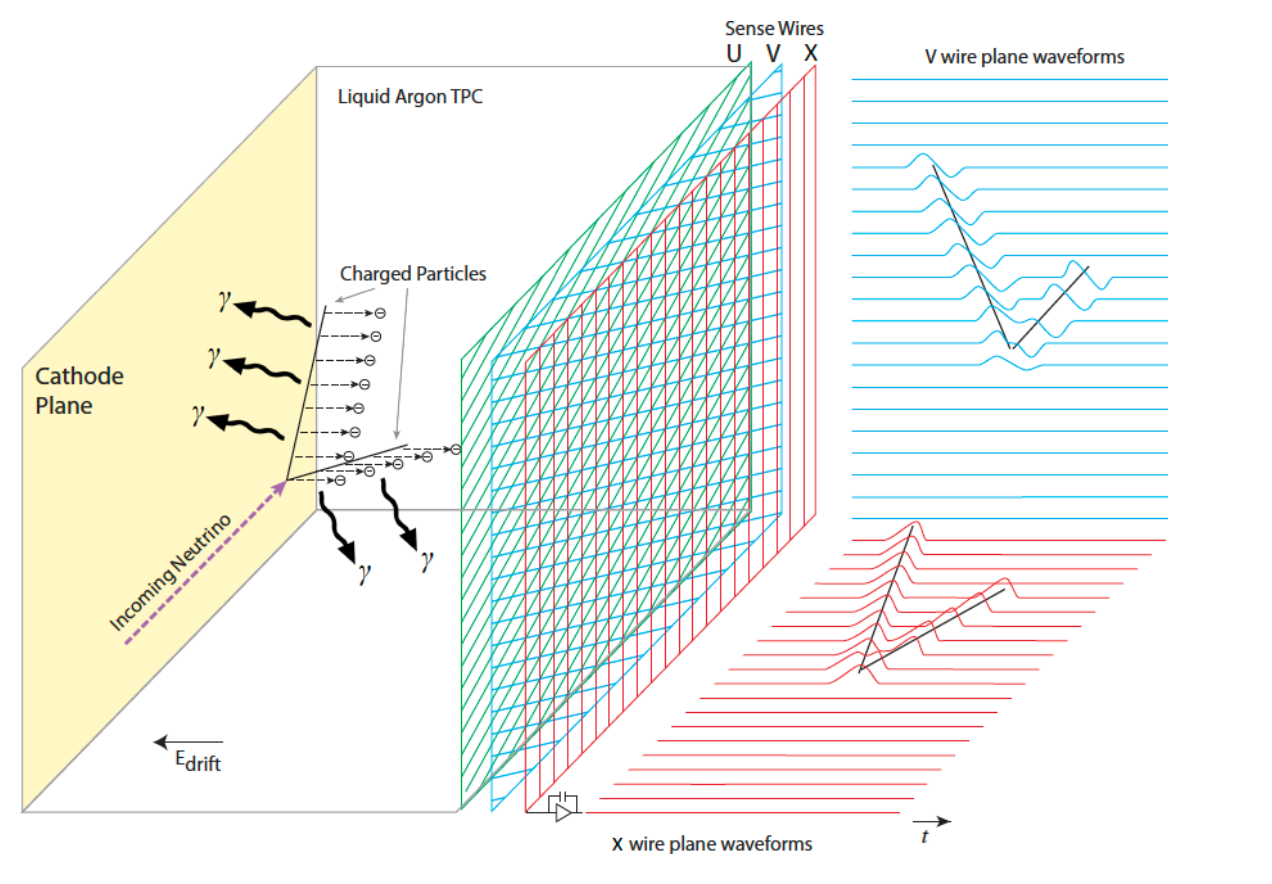
\includegraphics[width=.7\textwidth]{images/LArTPC.png}
		\caption{Source: \href{https://arxiv.org/abs/2002.02967}{\color{blue} Introduction to DUNE. Vol 1}}
		\label{far_detector}
	\end{figure}
\end{frame}

\begin{frame}
	\frametitle{Data Collection: Time Projection Chamber}
	\begin{figure}[h!]
		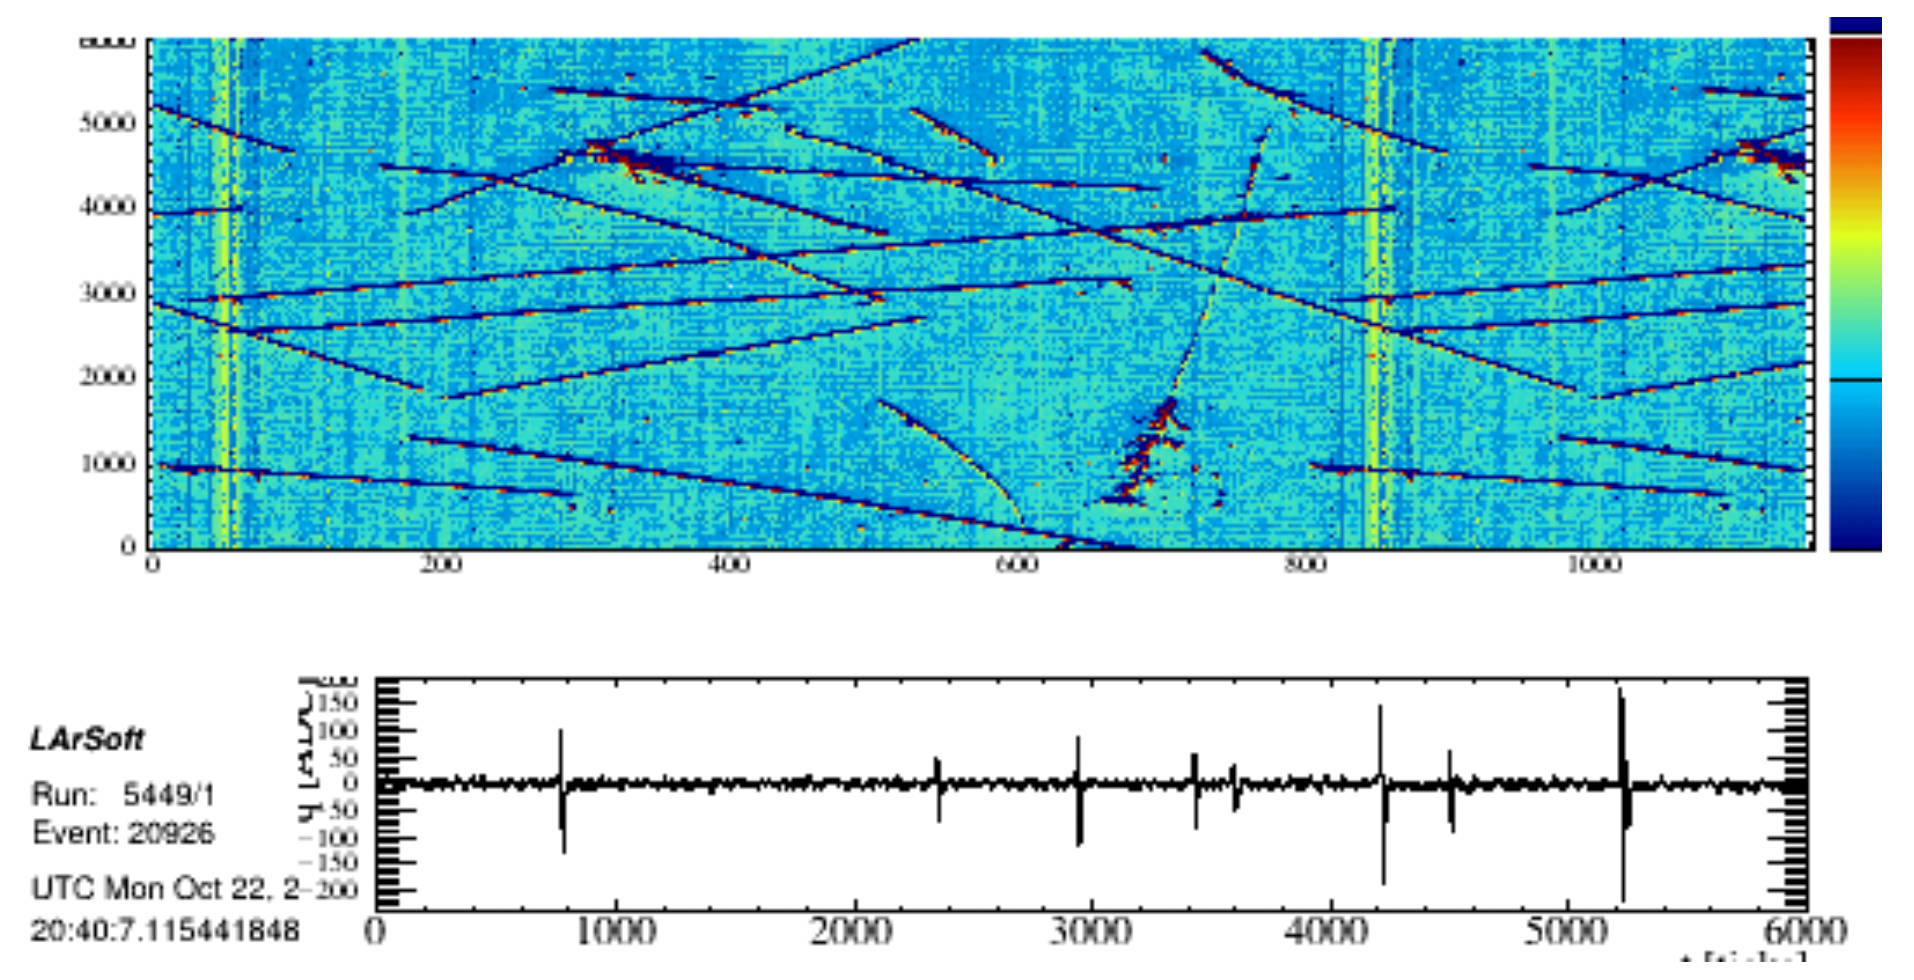
\includegraphics[width=.8\textwidth]{images/data1.png}
		\caption{Example of pedestal-subtracted data for one ProtoDUNE-SP wire plane. Source: \href{https://arxiv.org/abs/2002.02967}{\color{blue} Introduction to DUNE. Vol 1}}
		\label{far_detector}
	\end{figure}
\end{frame}

\begin{frame}
	\frametitle{Data Collection: Time Projection Chamber}
	\begin{figure}[h!]
		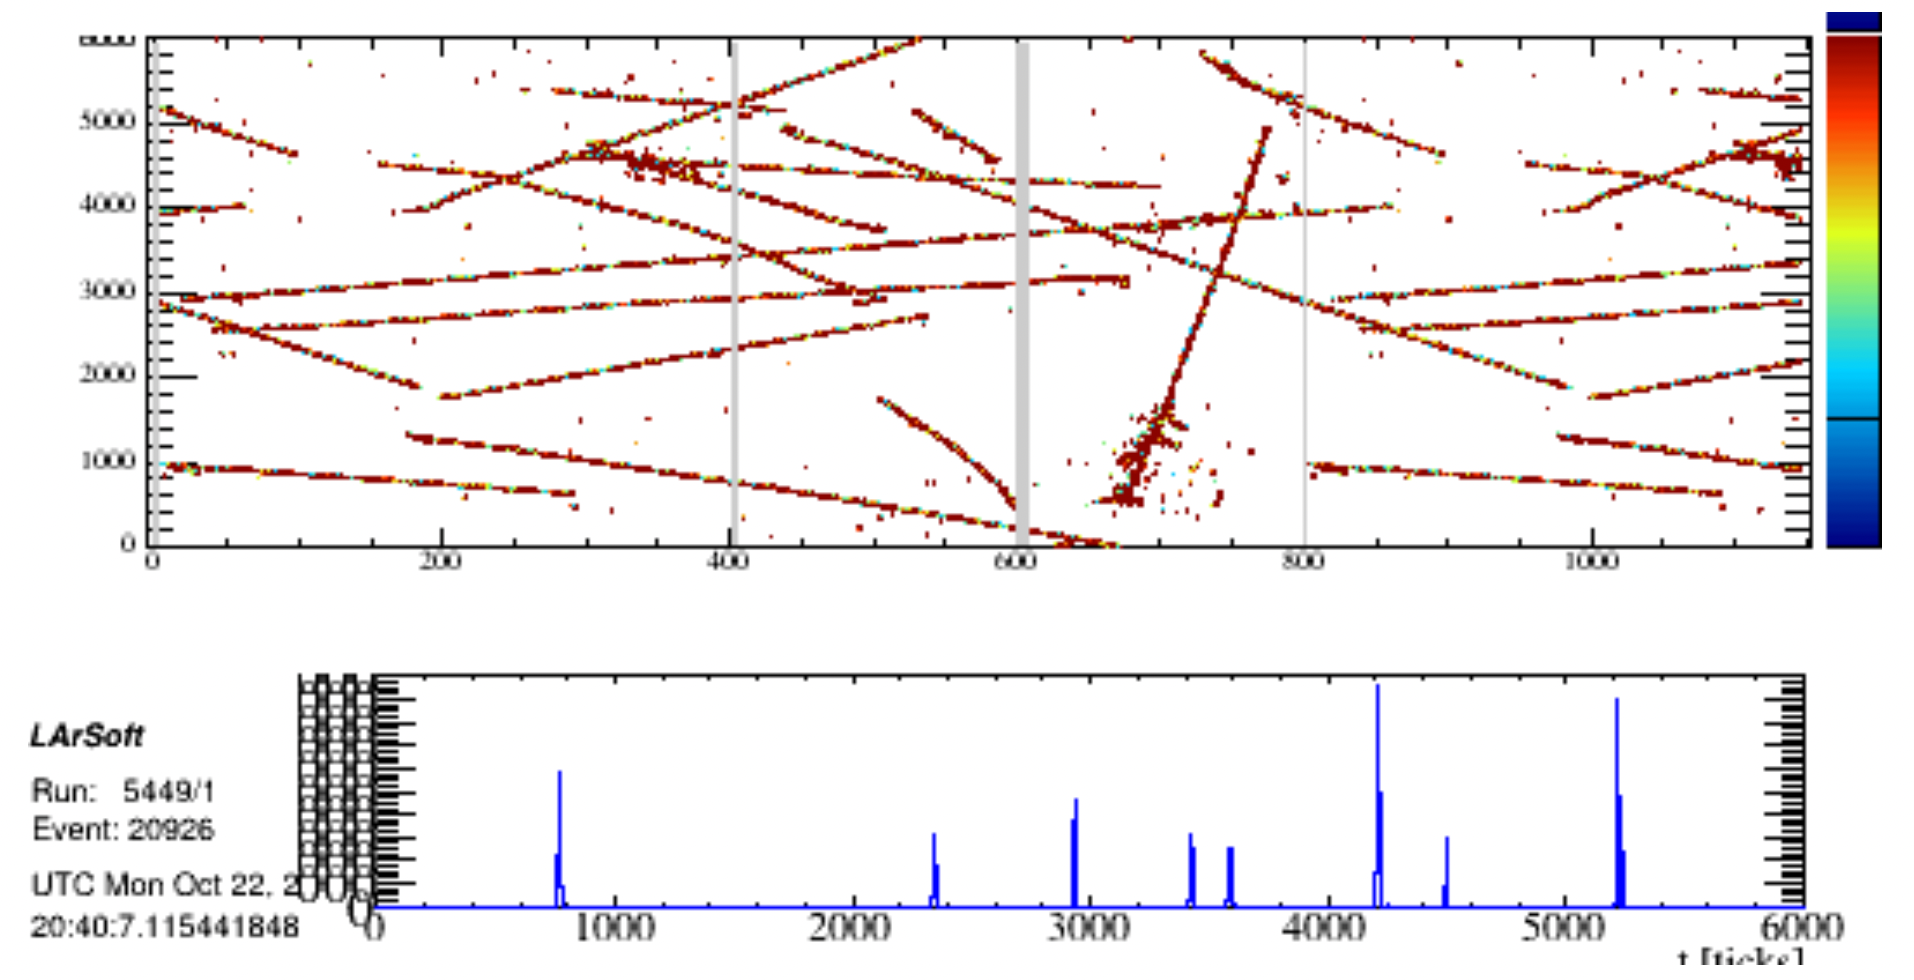
\includegraphics[width=.8\textwidth]{images/data2.png}
		\caption{Calibrated, deconvoluted pedestal-subtracted data for one ProtoDUNE-SP wire plane. Source: \href{https://arxiv.org/abs/2002.02967}{\color{blue} Introduction to DUNE. Vol 1}}
		\label{far_detector}
	\end{figure}
\end{frame}

% \begin{frame}
% 	\frametitle{Data Collection: Data Volumes}
% 	\begin{itemize}
% 		\item Single Phase:
% 		\begin{itemize}
% 			\item Each of the 150 SP anode plane assemblies has 2,560 readout channels
% 			\item Each is sampled with 12 bit precision every 500 ns
% 			\item Drift times approximately 2.5 ms, 6 GB per 5.4 ms readout window
% 		\end{itemize}

% 		\item Dual Phase:
% 		\begin{itemize}
% 			\item 153,600 readout channels and a full drift time of 7.5 ms
% 			\item Compressed size of a single ROI at 22 MB
% 			\item Gas amplification leads to a high S/N ratio (see previous slides)
% 		\end{itemize}
% 	\end{itemize}
% \end{frame}


% \begin{frame}
% 	\frametitle{Data Collection: ProtoDUNE}
% 	We have been training the model on ProtoDUNE samples.
% 	\begin{itemize}
% 		\item Consists of 6,000-15,000 12-bit, 0.5 $\mu$sec samples.
% 		\item Each 3 ms of APA readout consists of more than 15 M 16-bit values
% 		\item Data with a 7.5 ms window were also recorded.
% 	\end{itemize}
% 	Very computationally expensive.
% \end{frame}

\begin{frame}
	\frametitle{Data Collection: \texttt{.HDF5}}
	Each data sample collected in the LArTPC is processed and stored into an \texttt{hdf5} file.\\[0.20cm]

	To download an \texttt{hdf5} file to your local drive, run the following command:\\[0.20cm]

	\tiny{\texttt{scp [username]@computecanada.ca:projects/rpp-nilic/neutrino\_ml/MCprodW/[filename] /path/to/destination/on/local}}
\end{frame}


\begin{frame}
	\frametitle{Data Collection: \texttt{.HDF5}}
	\begin{figure}[h!]
		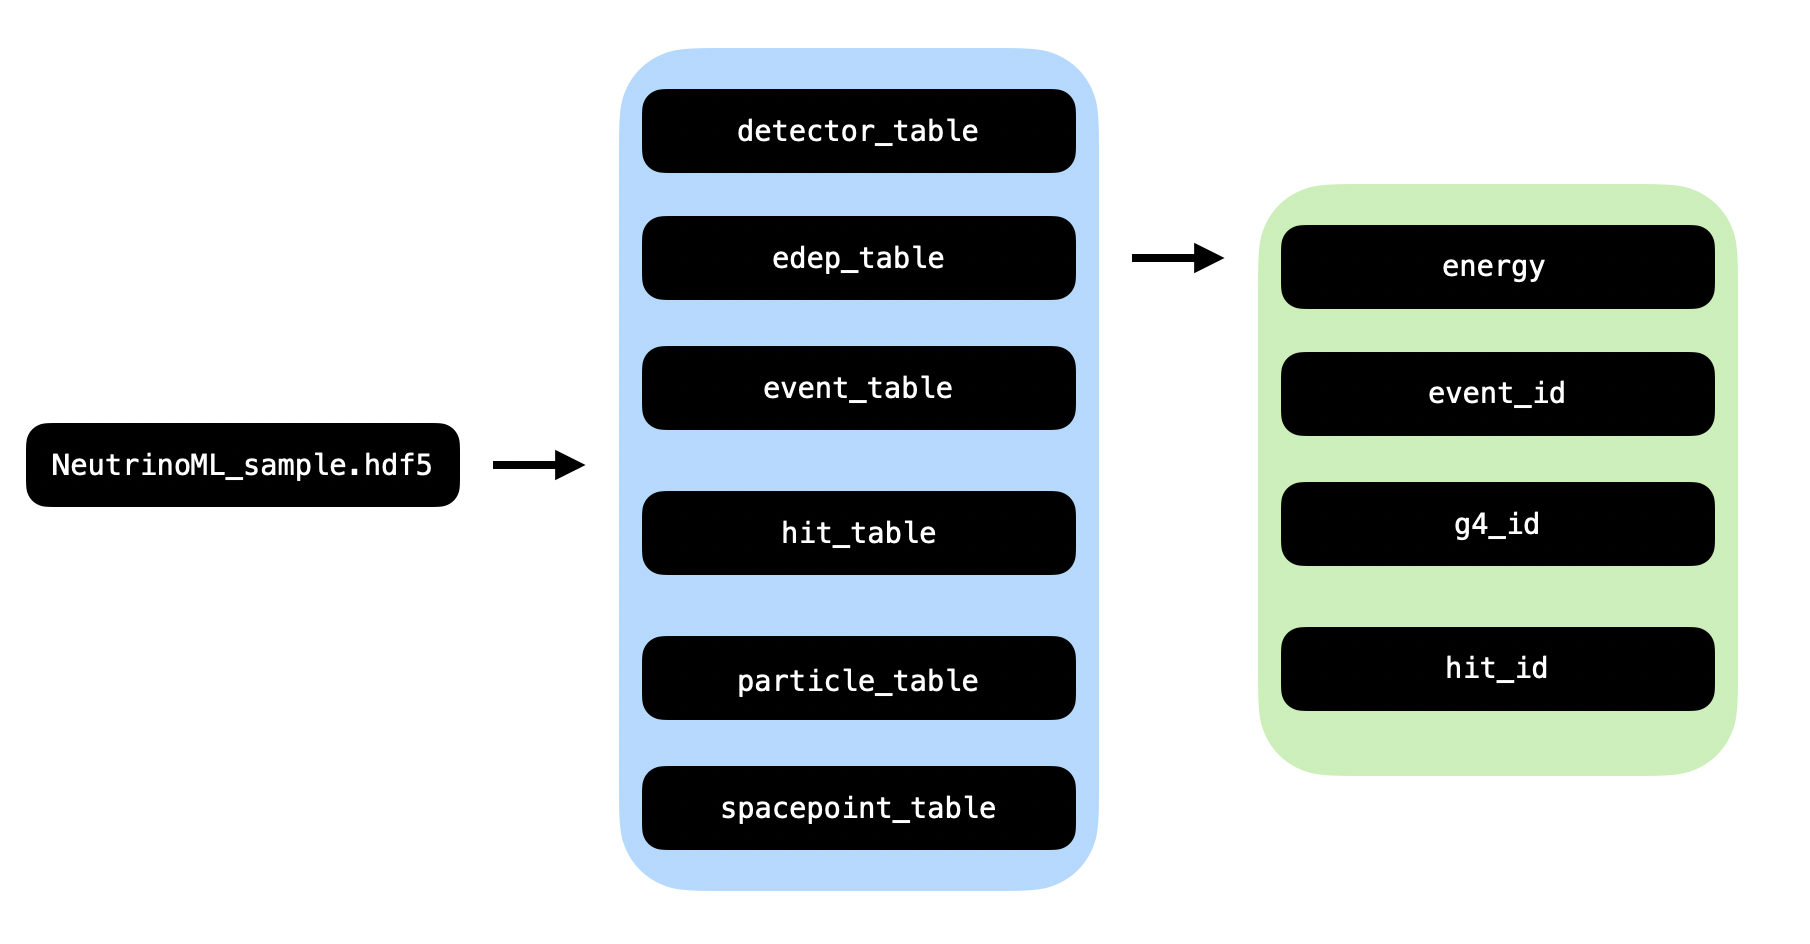
\includegraphics[width=.8\textwidth]{images/hdf5.png}
		% \caption{Calibrated, deconvoluted pedestal-subtracted data for one ProtoDUNE-SP wire plane. Source: \href{https://arxiv.org/abs/2002.02967}{\color{blue} Introduction to DUNE. Vol 1}}
		% \label{far_detector}
	\end{figure}
\end{frame}




\begin{frame}
	% This is where we discuss the specifics of NuGraph2.py. Need to go in detail about the way that the __init__ function operates (i.e. the encode, planenet, and nexusnet files followed by the decoder selection phase)
	\frametitle{Algorithm Structure}
		% The entire algorithm depends largely on three main components
		% \begin{enumerate} 
		% 	\item \texttt{train.py}
		% 		\begin{itemize}
		% 			\item This Python file takes as input the model parameters and the \texttt{hdf5} data file to be trained. 
		% 			\item Utilizes PyTorch library
		% 			\item Configures the model based on the input parameters (i.e. batch size, epoch, input/hidden features, etc...)
		% 			\item trains the model using the provided data set.
		% 			\item Calls PyTorch lightning Trainer module to train the model.
		% 			\item It calls the following two files;
		% 		\end{itemize}

		% 	\item \texttt{NuGraph.py}
		% 		\begin{itemize}
		% 			\item This file contains all of the network's architecture.
		% 			\item Contains the key functions \texttt{\_\_init\_\_()}\texttt{forward()}, \texttt{training\_step()}, \texttt{validation\_step()}, etc. which are passed to PyTorch LightningModule and utilized by the training module.
		% 		\end{itemize}

		% 	\item \texttt{H5DataModule.py}
		% \end{enumerate}
		\begin{figure}[h!]
			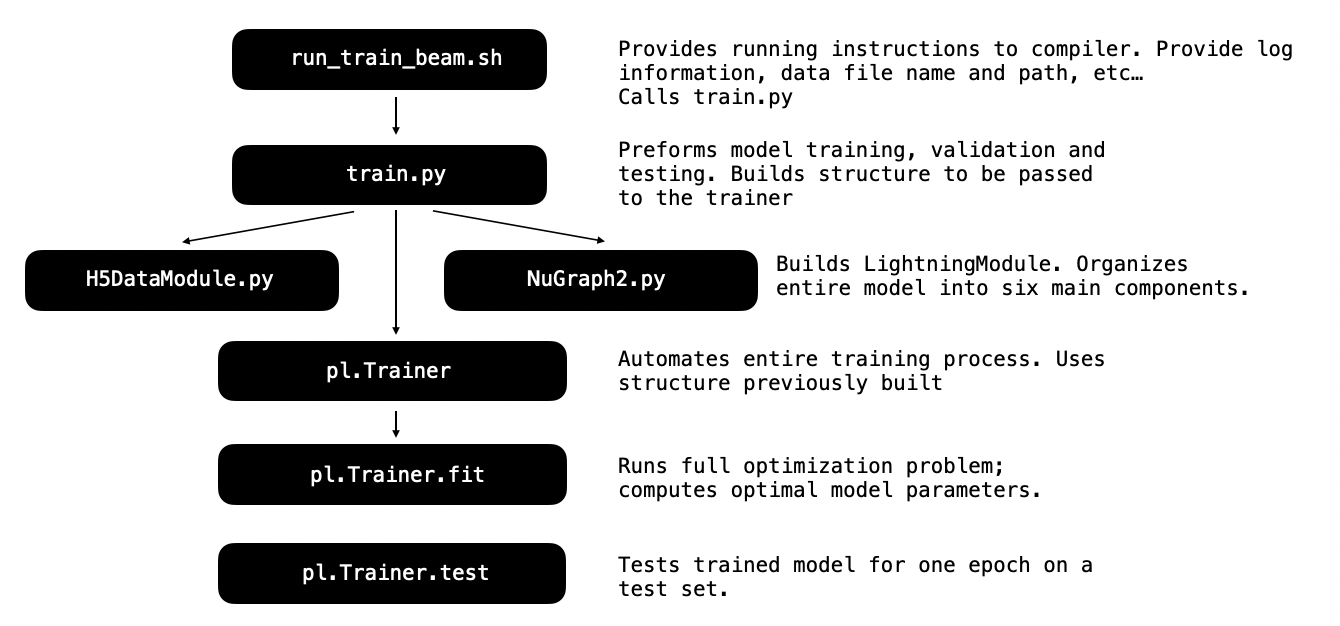
\includegraphics[width=1\textwidth]{images/model1.png}
			\caption{Description of NuGraph Neural Network. See \href{https://lightning.ai/docs/pytorch/stable/common/lightning\_module.html}{\color{blue} LighningModule}} for further documentation.
			\label{model1}
		\end{figure}
\end{frame}


\begin{frame}
	% This is where we discuss the specifics of NuGraph2.py. Need to go in detail about the way that the __init__ function operates (i.e. the encode, planenet, and nexusnet files followed by the decoder selection phase)
	\frametitle{\texttt{NuGraph2.py} Structure}
		\begin{figure}[h!]
			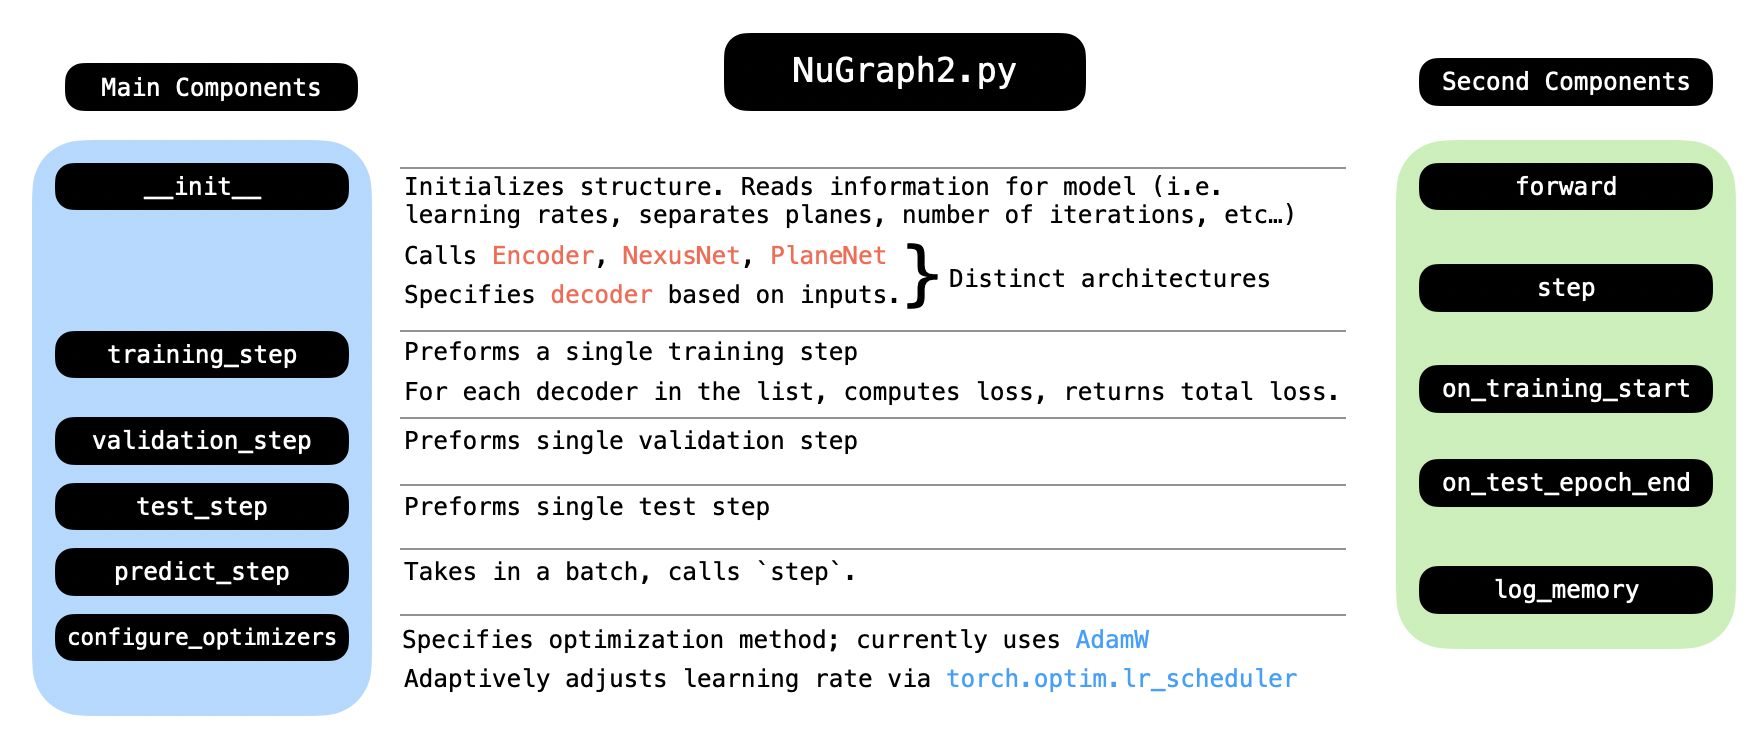
\includegraphics[width=1\textwidth]{images/model2.png}
			\caption{See \href{https://pytorch.org/docs/stable/generated/torch.optim.AdamW.html}{\color{blue} AdamW}}, \href{https://pytorch.org/docs/stable/generated/torch.optim.lr_scheduler.OneCycleLR.html}{\color{blue} \texttt{OneCycleLR}}.
			\label{model2}
		\end{figure}
\end{frame}


\begin{frame}
	% This is where we discuss the specifics of NuGraph2.py. Need to go in detail about the way that the __init__ function operates (i.e. the encode, planenet, and nexusnet files followed by the decoder selection phase)
	\frametitle{\texttt{Layer Description}}
		\begin{figure}[h!]
			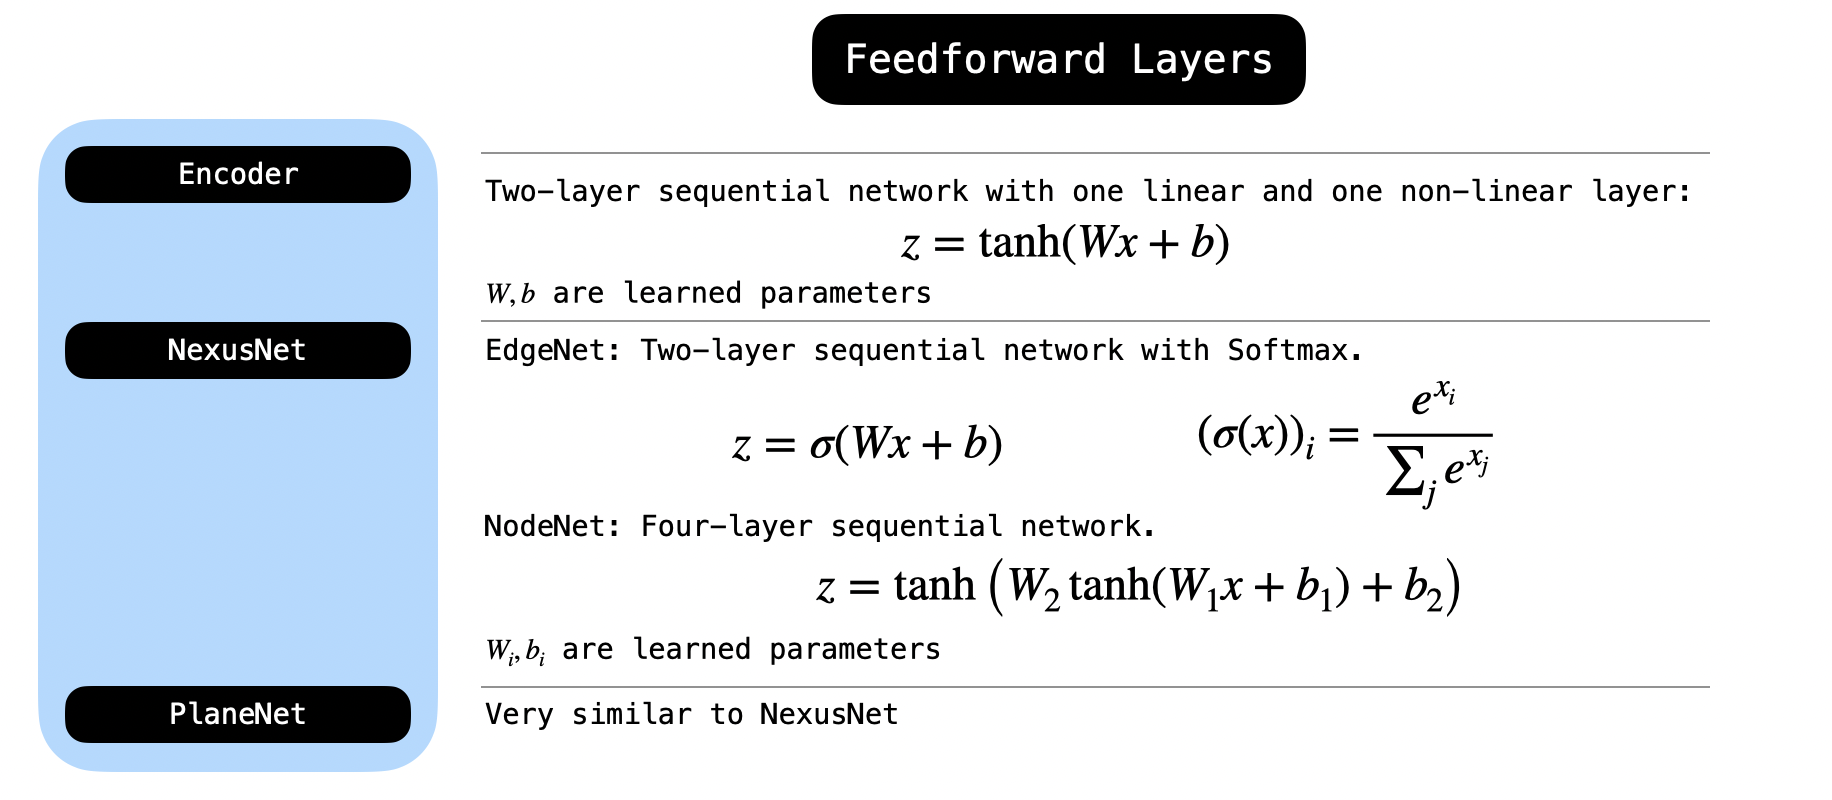
\includegraphics[width=1\textwidth]{images/model3.png}
			% \caption{See \href{https://pytorch.org/docs/stable/generated/torch.optim.AdamW.html}{\color{blue} AdamW}}, \href{https://pytorch.org/docs/stable/generated/torch.optim.lr_scheduler.OneCycleLR.html}{\color{blue} \texttt{OneCycleLR}}.
			\label{model3}
		\end{figure}
\end{frame}

\begin{frame}
	% This is where we discuss the specifics of NuGraph2.py. Need to go in detail about the way that the __init__ function operates (i.e. the encode, planenet, and nexusnet files followed by the decoder selection phase)
	\frametitle{\texttt{Decoder Descriptions}}
		\begin{figure}[h!]
			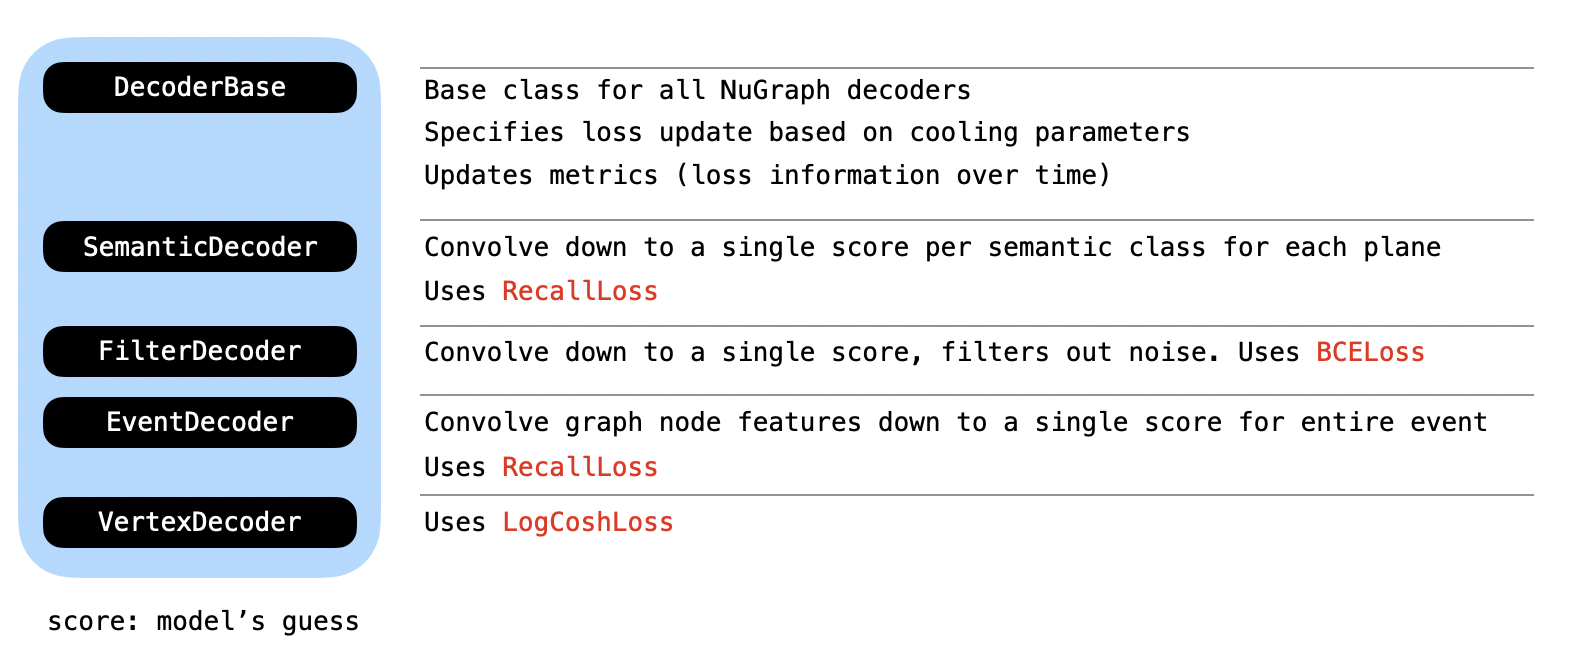
\includegraphics[width=1\textwidth]{images/decoders.png}
			% \caption{See \href{https://pytorch.org/docs/stable/generated/torch.optim.AdamW.html}{\color{blue} AdamW}}, \href{https://pytorch.org/docs/stable/generated/torch.optim.lr_scheduler.OneCycleLR.html}{\color{blue} \texttt{OneCycleLR}}.
			\label{decoders}
		\end{figure}
\end{frame}


\begin{frame}
	% This is where we discuss the specifics of NuGraph2.py. Need to go in detail about the way that the __init__ function operates (i.e. the encode, planenet, and nexusnet files followed by the decoder selection phase)
	\frametitle{\texttt{Loss Functions}}
		\begin{figure}[h!]
			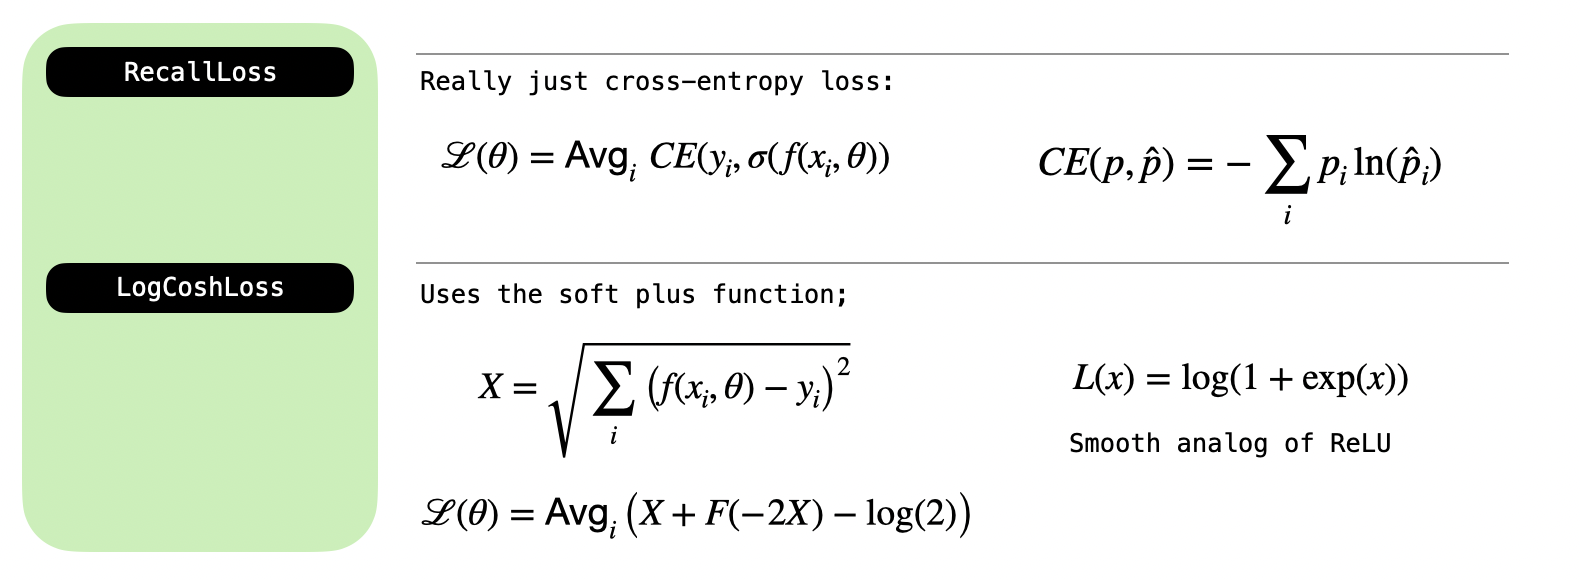
\includegraphics[width=1\textwidth]{images/loss.png}
			% \caption{See \href{https://pytorch.org/docs/stable/generated/torch.optim.AdamW.html}{\color{blue} AdamW}}, \href{https://pytorch.org/docs/stable/generated/torch.optim.lr_scheduler.OneCycleLR.html}{\color{blue} \texttt{OneCycleLR}}.
			\label{loss}
		\end{figure}
\end{frame}


% \begin{frame}
% 	% This is where we discuss the specifics of NuGraph2.py. Need to go in detail about the way that the __init__ function operates (i.e. the encode, planenet, and nexusnet files followed by the decoder selection phase)
% 	\frametitle{NuGraph Architecture}
% 		The NuGraph neural network architecture consists of three major components
% 		\begin{enumerate} 
% 			\item 

% 			\item 
% 		\end{enumerate}
% \end{frame}

\begin{frame}
	\frametitle{\texttt{H5Dataset.py \& H5DataModule.py} Description}
	
	\begin{itemize}
		\item H5Dataset.py defines a class which represents neutrino decay data sets
		\item H5DataModule.py also defines a similar data class based on the PyTorch LightningDataModule (inheritance from the LightingDataModule)
	\end{itemize}
\end{frame}


\section{Binary Classification of Decay Events}

\begin{frame}
\frametitle{Building Training Data}
	\begin{itemize}
		\item New training data will need to be configured as follows:
			\begin{itemize}
				\item Event follows the decay mode we are interested in
				\item Event does not follow the decay mode we are interested in
			\end{itemize}
		\item This configuration can be done by looking at the physical characteristics (e.g energy, momentum, spin) which can be found in the existing data
		\item Create a script to classify decay events of interest from existing data
			\begin{itemize}
				\item Once classified, attach a label (e.g 1 $\rightarrow$ decay of interest has happened, 0 $\rightarrow$ decay of interest has not happened) and send to new training model
			\end{itemize}
	\end{itemize}
\end{frame}


\begin{frame}
\frametitle{Pion Decay Modes}
	\begin{itemize}
		\item Focus will be on looking for decays modes involving $\tau$, $\nu_{\tau}$ (+ other particles), and Pions
		\item Current plan is to look for Pion decay modes with the correct spins
		\item We are going to look into this more starting this week
	\end{itemize}
\end{frame}




\section{Model Implementation}

\begin{frame}
\frametitle{Model Adjustments}
	\begin{itemize}
		\item Alter model to be able to handle this new class of data

		\item Reconfigure \texttt{H5DataModule.py}
		\item Choose ideal architecture (i.e. mimic \texttt{NexusNet, PlaneNet, etc...})
		\item Choose ideal loss function (i.e CE? LogCosh?)
	\end{itemize}
\end{frame}




\end{document}
